\begin{comment}
- Problem Formulation
	-- Physics Abstraction
	-- ALMA like Data
	-- Need of Synthetic Data
	-- Algorithm Input
	-- Algorithm Output
	
- Data Origin
    -- Splatalogue. What is it?
    -- Splatalogue. What allows to know?
    -- ASYDO. What is it?
    -- Simulation Features (and simplifications)
    -- First View to Predition Validation (We know the simulated lines present)
    -- ASYDO Parameters; Algorithm Parameters
    -- Redshift types
    -- Noise in each Band
    -- Line width
\end{comment}

% Data Origin
\section{Data} \label{sec:data_origin}
 
\subsection{Synthetic data}
% Need of Synthetic Data
% La solución que proponemos no depende de la quimica o fisica subyacente, por lo que es necesaria una cantidad suficiente de datos para encontrar patrones en la detección de líneas.
The solution proposed does not rely on underlying physics or chemistry, so it need enough data to find line-detection patterns.
At this time, available spectral data from ALMA is not enough, hence the use of synthetic data is necessary.

% Algorithm Input
% Synthetical data is generated through the simulation of data cubes with chemical components belonging to certain known group of isotopes.
% Algorithm Output
% The algorithm, only analyzing the spectra of this data cubes, gives a list with probability distribution of isotopes that could have generated the observed lines.
% With the simulated data, the actual lines that are present in the spectra can be known, so each prediction made by the classifier can be validated.

In the next section, the tools to get synthetic data are introduced and also, its use in this project.

% Splatalogue. What is it?
\subsection{Splatalogue. Catalogue of theoretical lines}
Splatalogue is the most up-to-date and complete spectral line database.
%
It consists in a catalog of experimental lines that gives a list of all known frequency for isotopes at their different known transitions states \citep{remijan_splatalogue:_2008}.
%
It aims to contain all known emission line data currently archived from labs all over the world - Jet Propulsion Laboratory (JPL), The Cologne Database for Molecular Spectroscopy (CDMS) \citep{muller_cologne_2005}, Lovas National Institute of Standards and Technology (NIST), among others sources \citep{remijan_splatalogue_2010}.

% Splatalogue. What allows to know?
Also, it allows to filter and search for spectral lines by isotope and wavelength ranges.
This tool is important for this work, since it is used to create the dictionary.

% ASYDO. What is it?
\subsection{ASYDO. Synthetic data}

The Astronomical Synthetic Data Observations (ASYDO) package \footnote{\url{https://github.com/ChileanVirtualObservatory/ASYDO}} is used to simulate ALMA-like data.
The simulation generates a training set to develop and test identification accuracy.
    
\begin{figure}
	\begin{center}
		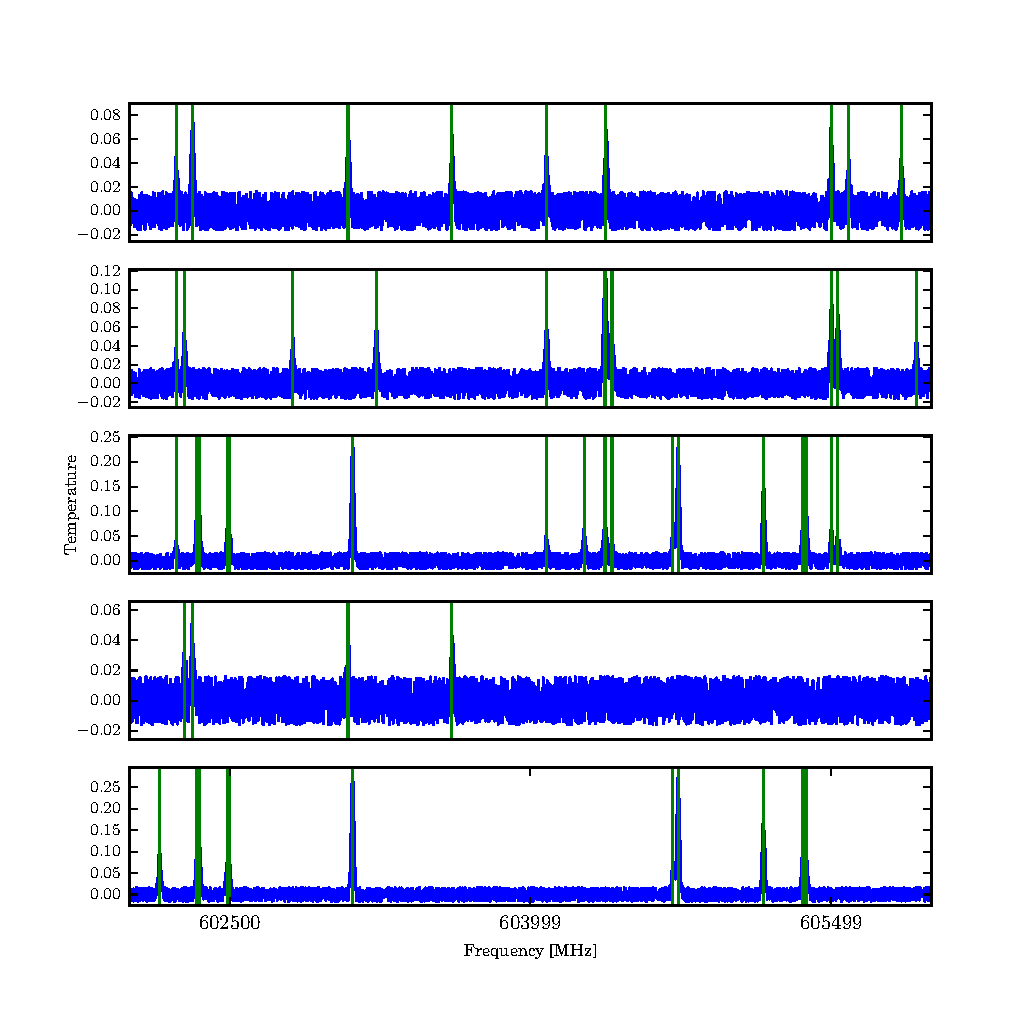
\includegraphics[width=0.45\textwidth]{images/overview}
		\caption{Example of ASYDO simulated spectra. Green vertical lines correspond to theoretical isotope lines used for the simulation.}
	\end{center}
	\label{fig:overview}
\end{figure}
    
% ASYDO Parameters
ASYDO can create fits files containing simulated hypothetical stellar objects using the next parameters:
%
\begin{easylist}[itemize]
& \textbf{Isolist}     : subset isotope list to generate a cube
& \textbf{Parameters}
&& \textbf{freq}         : spectral center (MHz)
&& \textbf{spe\_res}     : spectral resolution (MHz)
&& \textbf{spe\_bw}      : spectral bandwidth (MHz)
&& \textbf{(fwhm}, \boldmath{$\alpha$} \textbf{-skew}): skew-normal distribution parameters (MHz, parameter)
\end{easylist}

Skew-normal function gives form to spectral lines, in which $fwhm$ is full width at half maximum, and $\alpha-skew$ is its kurtosis parameter.
If $\alpha-skew = 0$, it degenerates to a Gaussian function, if $\alpha-skew < 0$, it is left-biased and $\alpha-skew > 0$, a right bias.

% Redshift types
We assume object movement redshift as known and corrected. 
A previous step is necessary to identify a set of stronger lines in the spectra and determine velocity shift \cite{sharpee_introducing_2003}.
Eliminating general redshift just left two error margins for observed frequencies: noise and internal redshift given by rotation and internal movements.

% Noise in each Band
Each band has different noise because of both radio-telescope sensitivity at each band, and nature of spectra signals at different wavelengths.

% Line width
The width of each line depends on skew-normal parameter $fwhm$.
For testing purposes, we modified the width in a 4 MHz range with a modification of ASYDO, incorporating this randomness to use different width for each spectral line.
The parameters we use for simulations are: both \textbf{alpha} and \textbf{delta} as 0 $degrees$, \textbf{spe\_res} of 1 $MHz$, \textbf{spe\_bw} as 4000 $MHz$ and \textbf{(fwhm}, \boldmath{$\alpha$} \textbf{-skew}) as $(8, 0)$.

